\subsection{Event Selection \& Analysis Regimes}\label{sec-regimeCat}
The trigger selections of the \vhb and \vhc resolved have been harmonised for the combined analysis, and are specified per lepton channel in 0-lepton (0L), 1-lepton (1L), and 2-lepton (2L). Further details on the trigger setup are given in Table \ref{aptab:trigs2015_to_2018} of the Appendix. In 0L, events are selected using the lowest un-prescaled \etm trigger, with increasing threshold rising from 70 GeV for data recorded in 2015, 90 to 110 GeV for 2016, and to 110 GeV for 2017 and 2018 due to higher trigger rate later in Run 3. The 1L channel triggers cover both the $e$ and the $\mu$ sub-channels. For the $e$-channel, single electron events must be triggered by the lwoest un-prescaled single electron triggers. For muons, the \etm trigger of 0L is used for events with \ptv > 150 GeV, while the lowest un-prescaled single muon trigger is used for events with a lower \ptv. Finally, the triggers for 2L are equivalent to 1L except for the muon channel where the \ptv threshold for switching between triggers is raised to 250 GeV. The use of \etm trigger at high \ptv for muons was shown to increase signal acceptancy by $\sim$ 5\%.\\

The different regimes of the analysis are defined by flavour tagging and the number of leptons in the final state. Jet flavour tagging is perhaps the most important part of the analysis. The Run 2 \gls{dl1r} tagger is used in the analysis for both $b$- and $c$-tagging. The so-called \glsfirst{pcft} scheme, shown in Figure \ref{fig:pseudotag}, to allow for a coherent joint definition and calibration of $b$- and $c$-tagged jets, adopting the technique first introduced for 2D $c$-taggin in the $VH(H\rightarrow c\bar{c})$ \cite{Collaboration:2721696}. For a given jet, it is first decided whether the jet is $b$-tagged ($B$), based on a $b$-tagging working point with 70\% efficiency\footnote{A 60\% \gls{wp} for $b$-tagging is first applied, but both are combined into the $B$-tagged category.}. If the $b$-tagging requirement is not met, it is then considered whether the jet is $c$-tagged using the same \gls{dl1r} tagger and two working points defined and calibrated for the purpose of the analysis. These working points are derived on a set of calibrating samples: dileptonic $t\bar{t}$ for $b$-jets, semileptonic $t\bar{t}$ for $c$-jets, and $Z$+jet samples for light-jets. A \textit{tight} ($T$) and a \textit{loose} ($L$) $c$-tagging requirements are defined and applied successively, each at an exclusive $c$-tagging efficiency of 20\%. Being made of the top tier $c$-jets, the $b$- and light-rejections of the tight $c$-tagging working point are improved compared to the looser working point. The $c$-jet (light-jet) efficiency in the $b$-tagged bins of the PCFT scheme is 7.85\% (0.181\%) and the $b$-jet (light-jet) efficiency in the loose $c$-tagged ($L$) bin is 11.5\% (6.5\%) while it is 4.5\% (0.9\%) in the tight $c$-tagged bin ($T$). Jets that are not tagged are ascribed the letter $N$. In the boosted regime, track-jet are ghost-associated to a given large-$R$ jet and are $b$-tagged in the \gls{pcft} scheme with a working point of 85\% efficiency. This very loose \gls{wp} was found to outperform the $X_{bb}$ tagger available at the time. While the analysis was underway, the superior \gls{dl1d} and GN-taggers introduced in Chapter \ref{chap-ftag} were not yet available as their calibration was an ongoing effort. Switching to a new tagger was not feasible from a practical point of view in the timing of the analysis. They represent, however, an exciting avenue for progress in future iterations of this search. \\ % check how the wp are defined

\begin{figure}[h!]
    \center
      \begin{minipage}[c]{0.69\textwidth}
        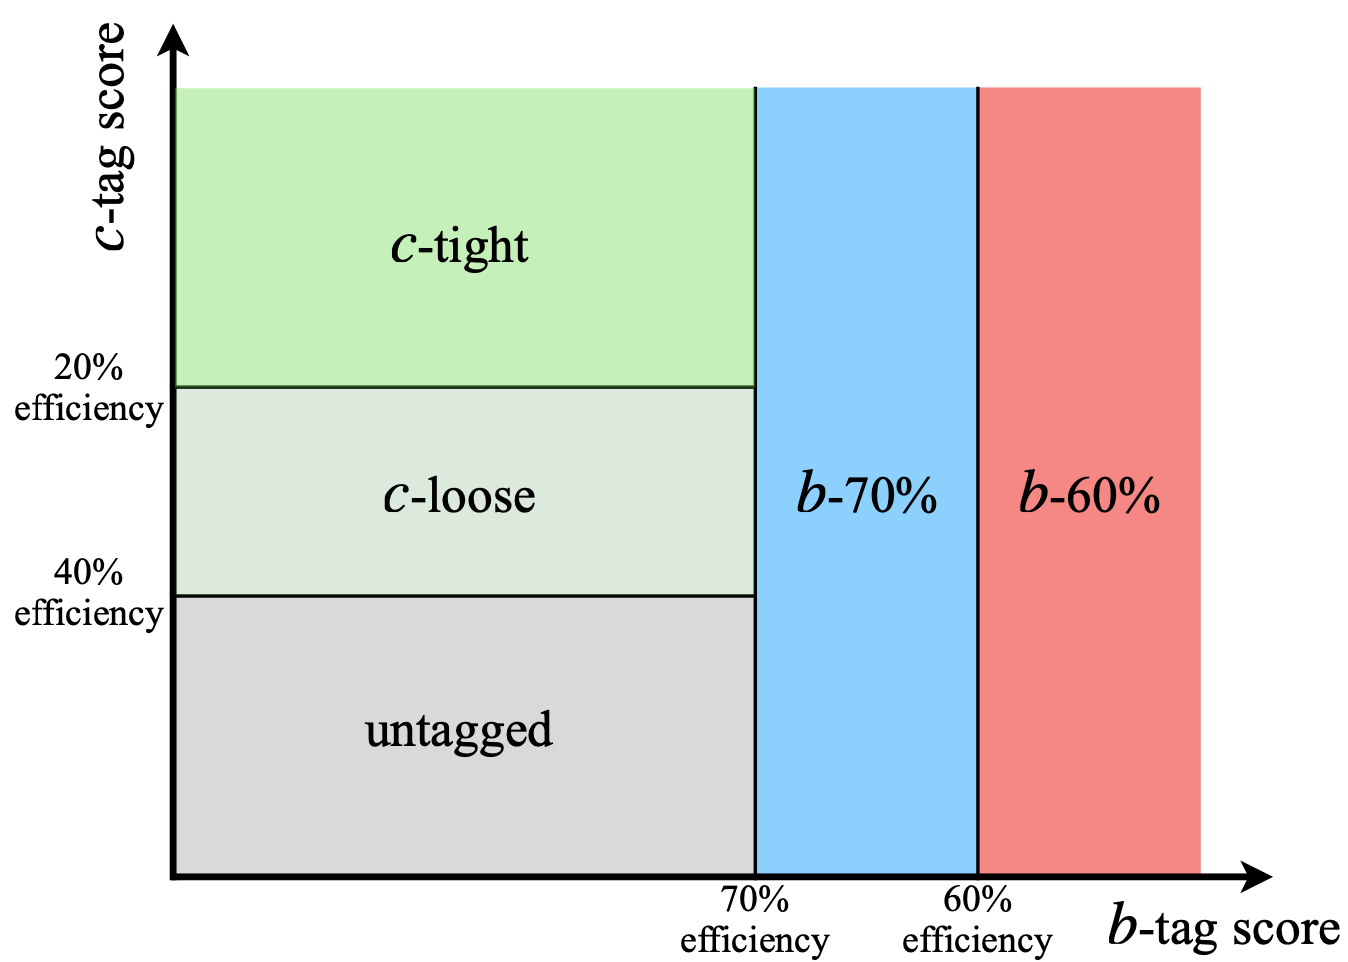
\includegraphics[width=0.98\textwidth]{Images/VH/pseudocontinuous.png}
      \end{minipage}
      \begin{minipage}[c]{0.3\textwidth}
        \caption{The \glsfirst{pcft} scheme, from the internal documentation. } 
        \label{fig:pseudotag}
      \end{minipage}
\end{figure}

In an event with at least two signal jets, the candidate jets selected to reconstruct the Higgs define an event-tag by combining their individual tags. Jets are selected using the so-called \textit{All Signal Jets} strategy, which was shown to improve the expected statistical significance. A hierarchy of tags is introduced, following: $B$ > $T$ > $L$ > $N$. The selected pair of candidates is made of the two signal jets having the highest tags, and the highest $p_T$ in case of ties. Events are labelled based on the tag of the selected jets, e.g., $TT$ is assigned to events with 2 tight $c$-tagged jet and $BL$ to events with a $b$-tagged and a loose $c$-tagged jets. 

\clearpage
%
% From: https://gitlab.cern.ch/atlas-physics-office/HIGG/ANA-HIGG-2020-20/ANA-HIGG-2020-20-INT1/-/blob/master/Tex/Texsection/Selection/VHbbccevSelTable.tex
\begin{table}[htbp]
    \begin{center}
    \begin{tabular}{C{6cm}|C{4cm}|C{4cm}}

    \hline \hline
    Resolved Analysis Regime & $VH(H\rightarrow b\bar{b})$ & $VH(H\rightarrow c\bar{c})$ \\
    \hline \hline
    \multicolumn{1}{c}{}  &\multicolumn{2}{c}{Common Selections}\\ \hline 
    Jets & \multicolumn{2}{c}{$\geq$ 2 signal jets}  \\
    Candidate jets tagging &  2 $B$-tags & $\geq1$ $T$-tag, no $B$-tag\footnote{The $V+l$ CR uses exactly one $L$-tag + one untag.} \\
    Leading Higgs ($H$) candidate jet $p_T$ & \multicolumn{2}{c}{$>$ 45 GeV} \\
    Sub-leading $H$ candidate jet $p_T$ & \multicolumn{2}{c}{$>$ 20 GeV} \\
    $m_{bb}$ or $m_{cc}$ & > 50 GeV (before correction) \\
    Non-$H$ candidate jet $p_T$ & \multicolumn{2}{c}{$>$ 30 GeV} \\ % TODO seems to be gone
    Candidate jets $\Delta R$  & \multicolumn{2}{c}{Upper cut $\Delta R \leq \pi(p_T^V)$} \\

    \hline \hline 
    \multicolumn{1}{c}{} &\multicolumn{2}{c}{0-Lepton} \\
    \hline
    Trigger & \multicolumn{2}{c}{$E_T^{\textrm{miss}}$ triggers} \\
    Jets & $\leq$ 4 jets & $\leq$ 3 jets \\
    Additional jets tagging & no $T$-tag & no $B$-tag \\
    Top CR tagging\footnote{\label{footnote-topCR}Candidate jet tagging ignored for the Top CR.} & \multicolumn{2}{c}{$\geq$1 $B$-tag + 1 $T$-tag} \\
    Leptons & \multicolumn{2}{c}{0 $VH$-loose lepton} \\
    $E_T^{\textrm{miss}}$ & \multicolumn{2}{c}{$>$ 150~GeV}  \\
    $E_{T, trk}^{\textrm{miss}}$  & - & $>$ 30~GeV \\
    $S_T = \sum_i p_T^{\textrm{jet}_i}$ & \multicolumn{2}{c}{$>$ 120 (2 jets), $>$150 GeV ($\geq3$ jets)}  \\ % Adapt: in object introduce S_T
    $m_T^W$ & \multicolumn{2}{c}{$>$ 10 GeV when $\geq$ 1 hadronic $\tau$} \\
    $|\textrm{min}\Delta \phi (E_T^{\textrm{miss}}, \textrm{jet})|$& \multicolumn{2}{c}{$>20\ensuremath{^\circ}$ (2 jets), $> 30\ensuremath{^\circ}$(3 jets)} \\
    $|\Delta\phi(E_T^{\textrm{miss}}, H)|$ & \multicolumn{2}{c}{$> 120\ensuremath{^\circ}$} \\
    $|\Delta\phi(j_1, j_2)|$ & \multicolumn{2}{c}{$< 140\ensuremath{^\circ}$} \\
    $|\Delta\phi(E_T^{\textrm{miss}},E_{T, trk}^{\textrm{miss}})|$ & \multicolumn{2}{c}{$< 90\ensuremath{^\circ}$} \\

    \hline\hline 
    \multicolumn{1}{c}{} & \multicolumn{2}{c}{1-Lepton} \\
    \hline
    Trigger &  \multicolumn{2}{c}{$e$-channel: single electron trigger} \\
            & \multicolumn{2}{c}{$\mu$-channel: single muon trigger ($p_T^V <$ 150 GeV)} \\
            & \multicolumn{2}{c}{and 0L $E_T^{\textrm{miss}}$ triggers} \\
    Jets & \multicolumn{2}{c}{$\leq$ 3 jets}  \\
    Additional jets tagging & no $T$-tag & no $B$-tag \\
    Top CR tagging\cref{footnote-topCR} & \multicolumn{2}{c}{$\geq$1 $B$-tag + 1 $T$-tag} \\ % TODO fix the footnoteref
    hadronic $\tau$-veto & \multicolumn{2}{c}{no hadronic $\tau$} \\ 
    Leptons & \multicolumn{2}{c}{1 $WH$-signal lepton} \\
            &  \multicolumn{2}{c}{$>1$~$VH$-loose lepton veto} \\
    $E_T^{\textrm{miss}}$   & \multicolumn{2}{c}{$>$ 30~GeV ($e$ channel)} \\
    $S_T$ & \multicolumn{2}{c}{$>$ 120 (2 jets), $>$150 GeV ($\geq3$ jets) (for $\mu$ with \etm trigger)}  \\ 
    $m_T^W$ & \multicolumn{2}{c}{$>$ 10 GeV for 75 < \ptv < 150 GeV} \\

    \hline\hline 
    \multicolumn{1}{c}{} & \multicolumn{2}{c}{2-Lepton}\\
    \hline
    Trigger &  \multicolumn{2}{c}{See 1L, \ptv $<$ 250 GeV for single $\mu$ trigger}\\
    Additional jets tagging & - & no $B$-tag \\
    Leptons & \multicolumn{2}{c}{2 $VH$-loose leptons} \\
            & \multicolumn{2}{c}{($\geq$ 1 $ZH$-signal lepton)} \\
            & \multicolumn{2}{c}{Same flavour, opposite-charge for $\mu\mu$} \\
    Top CR  & \multicolumn{2}{c}{Mixed $e\mu$ flavour} \\ 
    $m_{ll}$   & \multicolumn{2}{c}{81 $<$ $m_{ll}$ $<$ 101~GeV} \\
    %$E_T^{\textrm{miss}}$ significance (cut-based)  & \multicolumn{2}{c}{E_T^{\textrm{miss}}$/\sqrt{\textrm{HT}} < 3.5\sqrt{GeV}$} \\
    \hline\hline

    \end{tabular}
    \caption{Summary of the event selection in the 0-, 1- and 2-lepton channels of the resolved \vhb and \vhc regimes, adapted from the internal documentation. } % TODO ADAPT THE LEGEND FOR WHAT IS PRESENTED
    % There was also: Variables not presented in the text: $E_{T, trk}^{\textrm{miss}}$ is the missing transverse momentum calculated from the negative vector sum of the transverse momenta of tracks reconstructed in the inner detector and identified as originating from the primary vertex and $m_{ll}$ is the invariant mass of the di-lepton pair.
    \label{tbl:VHbbccevSelTable}
    \end{center}
\end{table}
%

\begin{table}[htbp]
    \hspace{-0.6cm}
    \begin{tabular}{C{2.8cm}|C{3cm}|C{2.5cm}|C{2cm}|C{2.5cm}|C{2cm}}
    \hline \hline
    Selection & 0-Lepton & \multicolumn{2}{c|}{1-Lepton} & \multicolumn{2}{c}{2-Lepton}  \\
    & & $e$-channel & $\mu$-channel & $e$-channel & $\mu$-channel \\ \hline \hline
    Trigger & \etm & Single electron & \etm & Single electron & \etm \\
    Leptons & 0 $VH$-loose lepton & \multicolumn{2}{c|}{1 $WH$-signal lepton} & \multicolumn{2}{c}{$\geq$ 1 $ZH$-signal lepton} \\
     & & \multicolumn{2}{c|}{No second $VH$-loose lepton} & \multicolumn{2}{c}{2 $VH$-loose leptons} \\
     &  & \multicolumn{2}{c|}{No hadronic $\tau$} & \multicolumn{2}{c}{Same flavour leptons} \\
     &  &  \multicolumn{2}{c|}{} & \multicolumn{2}{c}{Opposite charge for $\mu\mu$} \\ \hline
    \ptv &  \multicolumn{5}{c}{$>$ 400 GeV} \\
    Large-$R$ jet & \multicolumn{5}{c}{$\geq$ 1 large-$R$ jet ($R$ = 1.0), $p_T >$ 250 GeV, $|\eta| < 2$} \\
    Track-Jets & \multicolumn{5}{c}{$\geq$ 2 track-jets ($p_T > 10$ GeV, $|\eta| < 2.5$) matched to the leading large-$R$ jet} \\
    Tagging & \multicolumn{5}{c}{Exactly 2 of the 3 leading track-jets matched to the large-$R$ jet must be $b$-tagged} \\
    $m_J$ & \multicolumn{5}{c}{$> 50$ GeV} \\ \hline
    \etm & $>$ 250 GeV & $>$ 50 GeV & - & \multicolumn{2}{c}{-} \\ 
    $\min\Delta\phi(E_T^{\textrm{miss}}, \textrm{jets})$ & $> 30\ensuremath{^\circ}$ & \multicolumn{2}{c|}{-} & \multicolumn{2}{c}{-} \\
    $\Delta\phi(E_T^{\textrm{miss}}, H)$ & $> 120\ensuremath{^\circ}$ & \multicolumn{2}{c|}{-} & \multicolumn{2}{c}{-} \\
    $m_{ll}$ & - & \multicolumn{2}{c|}{-} &  \multicolumn{2}{c}{$66$ GeV $< m_{ll} < 116 $ GeV} \\ \hline \hline
    \end{tabular}
    \caption{Summary of the event selection in the 0-, 1- and 2-lepton channels of the boosted \vhb regime, adapted from the internal documentation.} % TODO ADAPT THE LEGEND FOR WHAT IS PRESENTED
    \label{tbl:VHbbBoostevSelTable}
\end{table}

\subsection{Event Categorisation}\label{sec-eventCat}
In all regimes, the number of reconstructed charged lepton defines three channels as the 0-lepton (0L), 1-lepton (1L), and 2-lepton (2L). Events are futher categorised following a successive decomposition into regions of defined tagged, vector boson $V$ transverse momentum $p_T^V$, and number of jets. A further categorisation on the angular separation $\Delta R(j_1, j_2)$ between the Higgs-candidate jets, defined in Equation \ref{eq-deltaR}
\begin{equation}\label{eq-deltaR}
    \Delta R(j_1, j_2) = \sqrt{(\eta_{j_1} - \eta_{j_2})^2 + (\phi_{j_1} - \phi_{j_2})^2 },
    \end{equation}
is used in the non-boosted regime to define an orthogonal \gls{cr} per \gls{sr} enriched in $V$+jets and $t\bar{t}$ backgrounds. This split is governed by a $p_T^V$ dependent cut on the $\Delta R$ that was derived to give a specific signal purity and diboson yield, as described in more details in Appendix \ref{ap-sec-vh-deltaR}. The categorisation gives rise to signal and control regions that enter the statistical analysis defined in the fit framework of Section \ref{sec-fitFramework}. \\ 

The resolved \vhb requires exactly 2 $b$-tagged jets ($BB$) and events are separated into a 2 and 3 jets region. In 0L and 2L, a 4 jets regions is included for more sensitive \gls{stxs} measurements\footnote{In bins with more than one additional jets.}, with the 0L being exactly made of 4-jets events to limit $t\bar{t}$ contamination and the 2L allowing 4 or more ($\geq 4$) jets. These regions are split in different bins of $p_T^V$ as [75, 150] GeV (except for 0L\footnote{It is not feasible in 0L due to the trigger threshold on $E_T^{\textrm{miss}}$}), [150, 250] GeV, and [250, 400] GeV. Finally, control regions are defined orthogonaly to each signal region utilising events with high $\Delta R$ between the Higgs-candidate jets (\textit{high-$\Delta R$ CR}) to measure the yield of $V$+jets and $t\bar{t}$ from data. An extra low-$\Delta R$ control region is used in 1L to better control the $W$ + $bb$ contribution.\\

The resolved \vhc adopts a similar event categorisation to the resolved \vhb, with now at least 1 tight c-tagged jet required for the signal region. The categorisation of the signal region is finer, splitting into one region with loose or tight $c$-tag to define the 2 $c$-tag in addition to the first tight $c$-tag, region and another region having an additional non-tagged jet $N$ (neither $b$- nor $c$-tagged) defining the 1 $c$-tag region. The $p_T^V$ bins are the same, except for the higgest $p_T^V$ one that is relaxed to $\geq 250$ GeV given the limited impact of the overlap of this regime with the boosted \vhb. The jet multiplicity is used to define a 2 and a 3 jets regions (the latter being 3 or more jets in 2L), where the latter includes at least 3 jets. Orthogonal \gls{cr}s to the \gls{sr}s include the \highdr. For 1L and 2L, additional \gls{cr}s are defined by selecting Higgs candidate jet with one loose $c$-tag and one untagged ($LN$) to constrain the significant $V$+light-jet ($V+l$) background\footnote{Except in the [75, 150] GeV $p_T^V$ region of 1L due to high statistics-related fit instabilities.}. The resolved \vhb and \vhc share a top control regions in similar \ptv and jet multiplicity bins as the \gls{sr}. In 0L and 1L, they are defined by requiring a one $b$-tag in combination with a one tight $c$-tag. In 2L, they are defined by requiring leptons of different flavours instead of the same flavour ($e\mu$).\\

For the boosted \vhb, there are two \ptv bins: [400, 600] GeV and $\geq$ 600 GeV. The \gls{sr}s are defined by requiring exactly two of the three leading subjets associated to a single learding large-$R$ jet to be $b$-tagged. A $t\bar{t}$ control regions is defined in 0L and 1L by migrating events with a $b$-tagged track jet outside the large-$R$ jet with an angular selection $\Delta R(\textrm{VR-track jet, large-}R\textrm{ jet}) > 1$. \\

A summary of the full event categorisation and the regions thus defined at the moment of writing is shown in the Figure \ref{fig:ana-strat-det} and a summary of the signal event selection is shown in Table \ref{tbl:VHbbccevSelTable} for the resolved regime and Table \ref{tbl:VHbbBoostevSelTable} for the boosted regime. This corresponds to the status of the analysis following the 3$^{\textrm{rd}}$ unblinding approval, that happened on the 18$^{\textrm{th}}$ January 2024. 

\clearpage

\begin{sidewaysfigure}[t!]
    \centering
    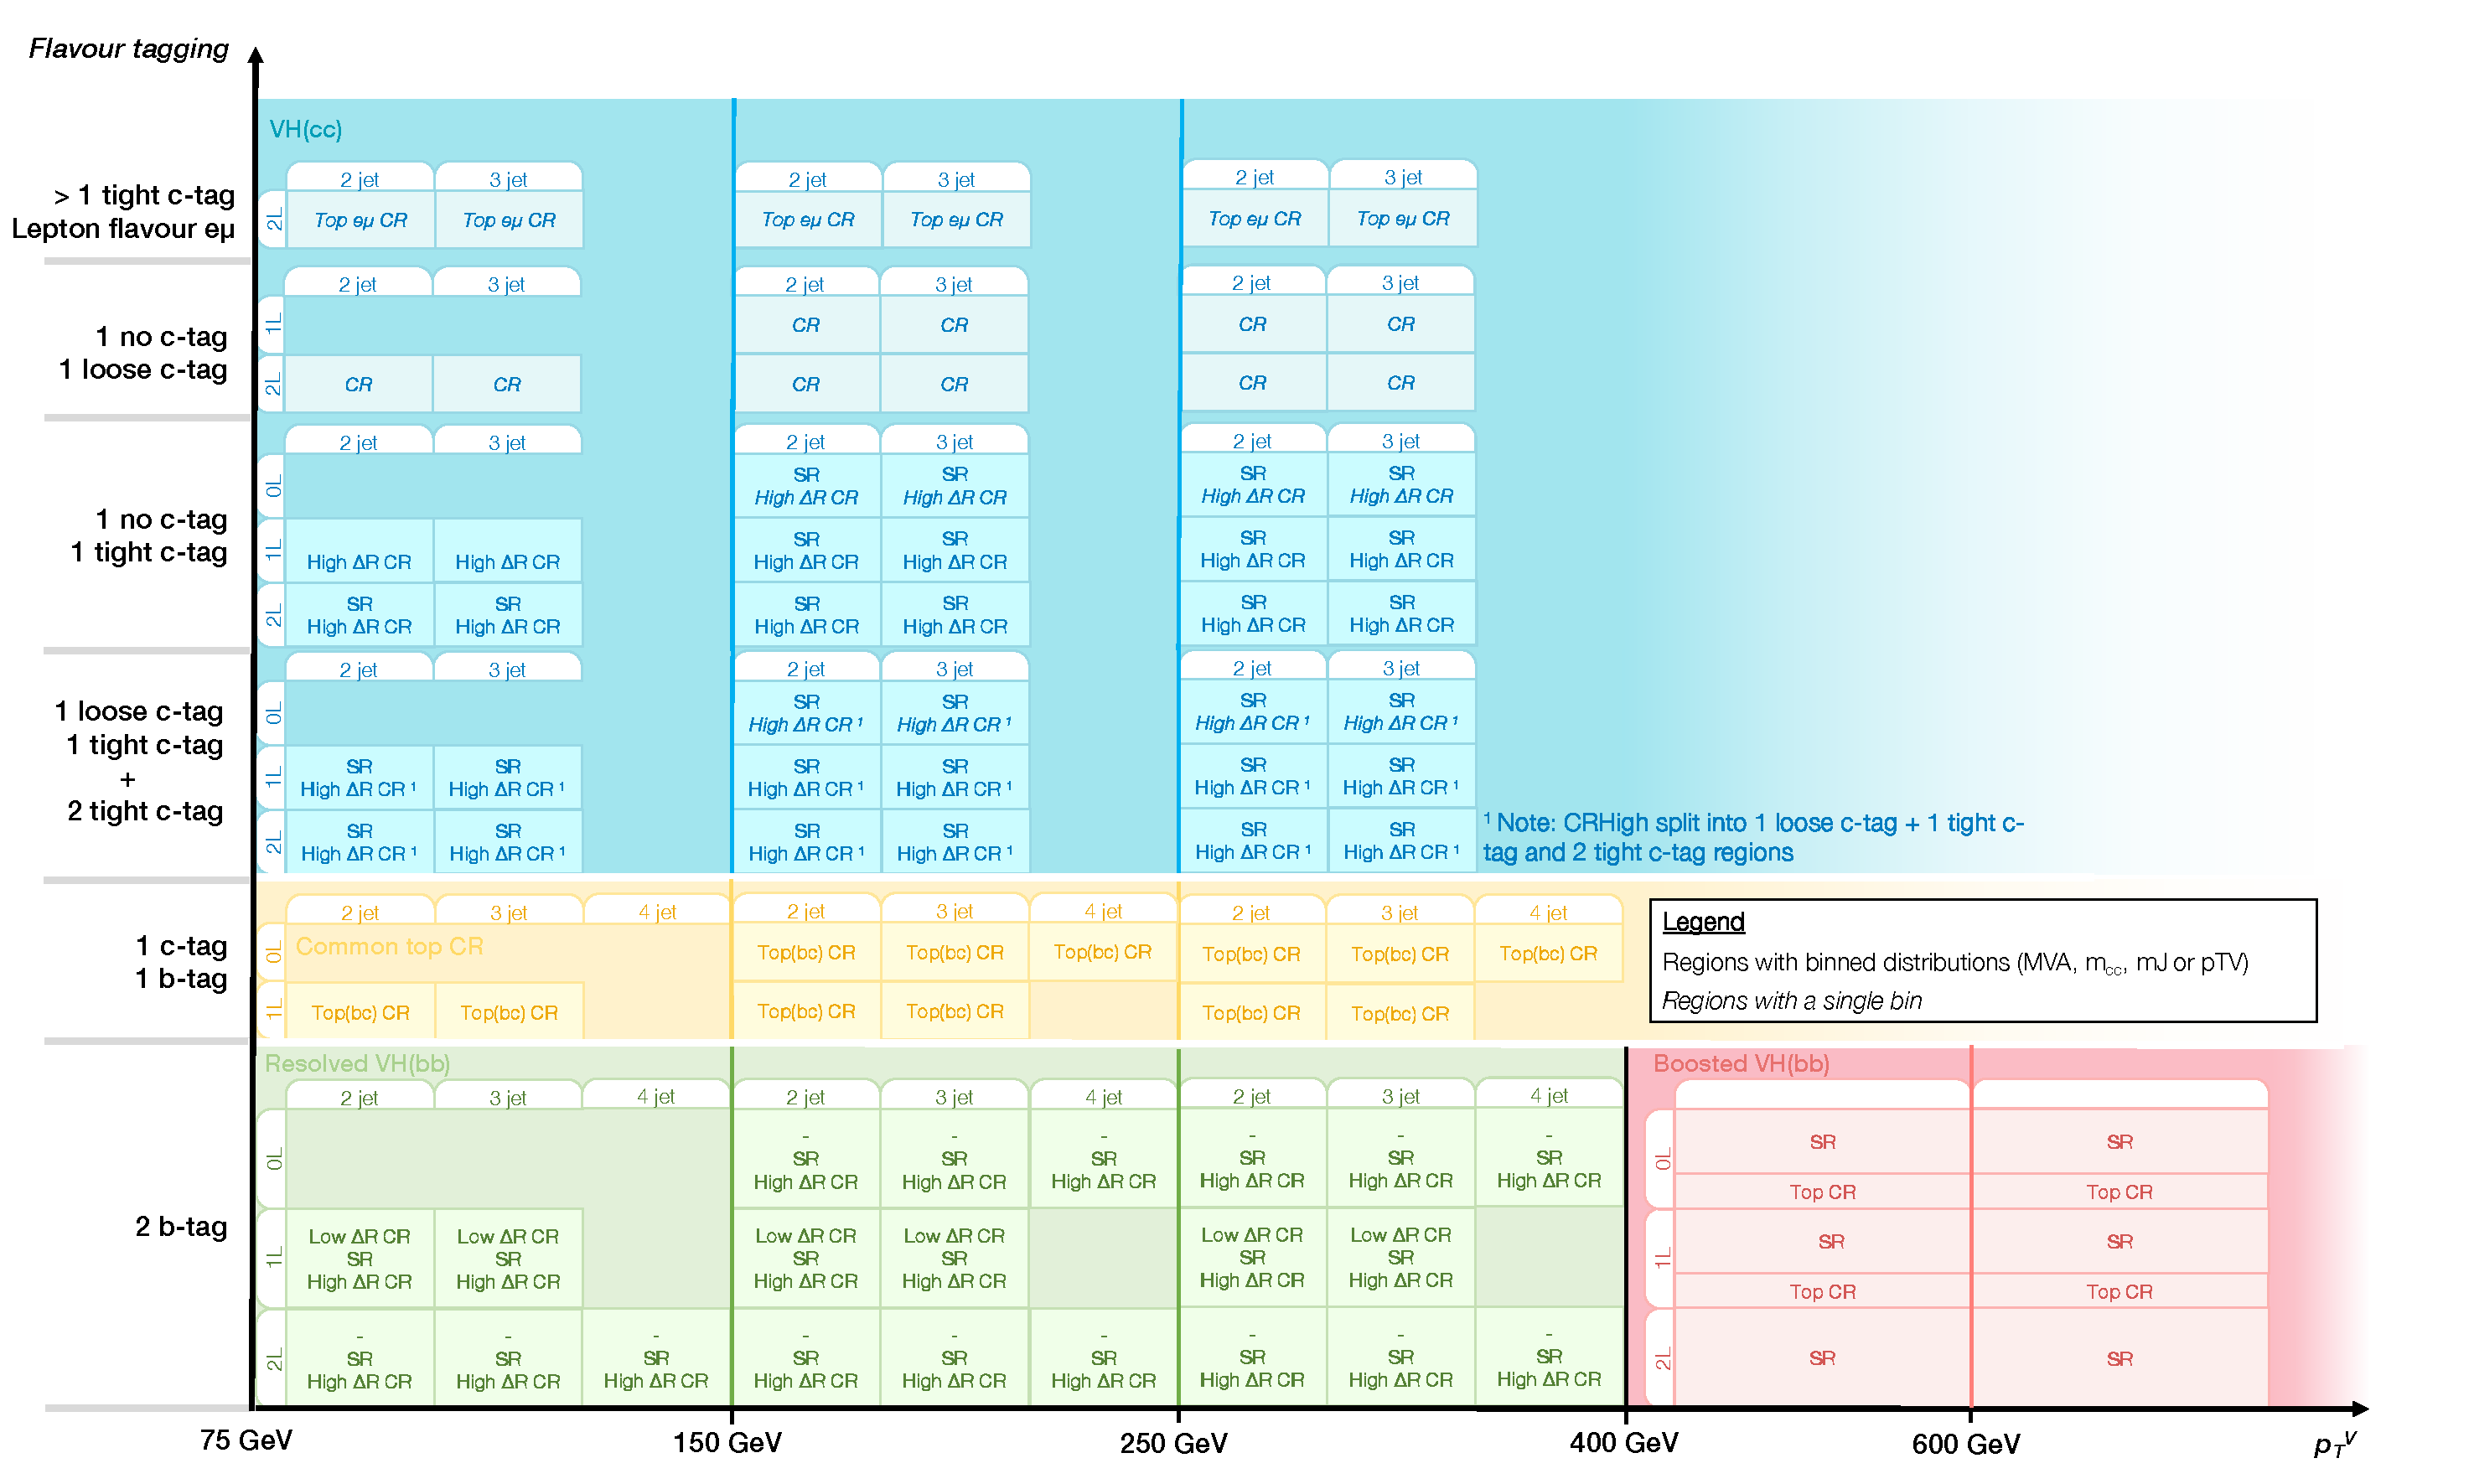
\includegraphics[width=\textwidth]{Images/VH/Cat/VH_analysis_cat.pdf}
    \caption{The current split of the analysis regions considered in the $VH (H\rightarrow b\bar{b}/c\bar{c})$ Combined Analysis, showing the Signal Region (SR), High and Low $\Delta R$ control region (CR), and the top CR. From the internal documentation.} 
    \label{fig:ana-strat-det}
\end{sidewaysfigure}


An important update to the $VH (H\rightarrow c\bar{c})$ analysis is the introduction of a \glsfirst{bdt} score distributions as discriminant variables instead of the invariant mass of the Higgs candidates jets $m_{c\bar{c}}$. The BDT is trained with kinematic and flavour information about the Higgs candidate jets as well as lepton information and higher-level variables such as angles between the objects, the sum of momenta, and the invariant mass. The algorithm provides a score in the [-1, 1] range corresponding to low or high signal probability and significantly enhances the background-signal separation of the analysis.

\subsection{Top Control Region}
The top control region (topCR) is used to constrain the rather significant top background that peaks at signal-like values of the discriminant variables. Indeed, when the candidate jets selected correspond to the $b$- and $c$-jet from a $t\bar{t}$ decay, the invariant mass of the pair peaks at 120 GeV, exactly the region of interest for a Higgs decay search. The topCR is defined by requiring at least one $c$-tagged jet in combination with at least one $b$-tagged jet using the \textit{AllSignal} strategy, as previously described. This tagging requirement renders it orthogonal to the signal region of the analysis and targets the decay topology of the different top processes: 
\begin{itemize}
\item Semi-leptonic $t\bar{t}$ decay: both $t$ follow the usual decay chain  $t \rightarrow b$ + $W$, with one of the $W$ decaying leptonically and the other one to a pair of quarks. Some events from this process can enter the signal region when some of the quarks are $c$-tagged or if the $b$-jets are mis-tagged or flew out of the detector acceptance. Requiring the combination of a $b$-tag and a $c$-tag effectively selects this process, the $b$ coming from the direct $t$ decay and the $c$ from a subsequent $W$ decay. 
\item Single top $t$-quark: predominantly the $Wt$ process $W$ $t \rightarrow W$ +  $b$ + $W$, with one $W$ decaying leptonically and the other hadronically. Some of these background events can enter the signal region if the $b$- is missed and if a jet is $c$-tagged, from the extra $W$ or if the $b$-jet is mis-tagged. Events from the single-top $t$- and $s$-channel of the process $t \rightarrow b$ + $W$ bring a smaller contribution, as the $c$-tagged jet must come from \textit{Initial State Radiation} (ISR) or \textit{Final State Radiation} (FSR) if the $b$ is not mis-tagged. Single-top is a minor background in 0L and 1L, with the main component being the production of $Wt$ pairs. The $t$-channel and $s$-channel contribute less than 1\% of the total background.
\end{itemize}

Of the two processes, the $t\bar{t}$ is therefore the most important one and a main background in the 0L and 1L channels. Due to their similarities, the $t\bar{t}$ and $Wt$ processes are considered as a single \textit{top} background in the analysis. In 2L, because this top background is small, no flavour-based topCRs are introduced and a different strategy is employed where the top is directly constrained in a pure top-$e\mu$ control region defined by requiring two charged leptons of different flavours. For the 0L and 1L channels, the expected top background normalisation and its kinematic distributions, as given by the MC simulation, are adjusted using data in the topCRs; this is extrapolated to the signal regions under consideration of extrapolation effects (and corresponding extrapolation uncertainties) that account for differences between the topCRs and SRs. \\

The combined top background is separated into different components, depending on the true flavour of the two candidate jets, that can be combined during the statistical analysis. These are:
\begin{itemize}
\item top($bb$): in this case, the two $b$-jets produced during the $t\bar{t}$ decay are selected. This is a small component in the signal regions of the $VH(H\rightarrow c\bar{c})$ analysis, due to the 70\% efficiency WP for $b$-tagging and the low mis-tag rate for $b$-jets in $c$-tagging. Naturally, in $VH(H\rightarrow b\bar{b})$ it is the leading contribution. Due to the origin of the candidate jets, a large $\Delta R_{b\bar{b}}$ is expected between the two $b$-jets so this component is most effectively constrained by the High $\Delta R$ CR. 
\item top($bc$): where the $b$ is from a $t$ decay and the $c$ from a subsequent $W$ hadronic decay (or from ISR/FSR though this is less likely). Given the definition of the topCR, this is the dominating component in that region and the most important to constrain in the signal regions of the $VH(H\rightarrow b\bar{b}/c\bar{c})$ analyses due to its signal-like kinematics. 
\item top($bl$): where $l$ stands for anything not $b$ nor $c$ (light jets predominantly but also some mis-tagged hadronic $\tau$). This component is similar to the top($bc$) as it also consists of a $b$ + a jet from the $W$ and can end up in the SRs and topCRs due to mis-tags.
\item top($lq$): where $l$ is as above and $q$ can be any sort of jet except a $b$. This is a small component that mostly accumulates in the background-like part of the BDT score distribution. It is not constrained in the high $\Delta R$ regions nor the topCRs.
\end{itemize}
The signal region distributions in the 1L channel in the $p_T^V$ range $[150, 250]$ GeV are displayed in Figure \ref{fig:SRslowptv}. While the top is not the dominant background, except in the tighter tagged TT 3-jet region, its relative contribution to the background composition increases at signal-like values of the discriminant, as shown in Figure \ref{fig:topContentSR}. \\

\begin{figure}[h!]
%\hspace{-2.0cm}
\center
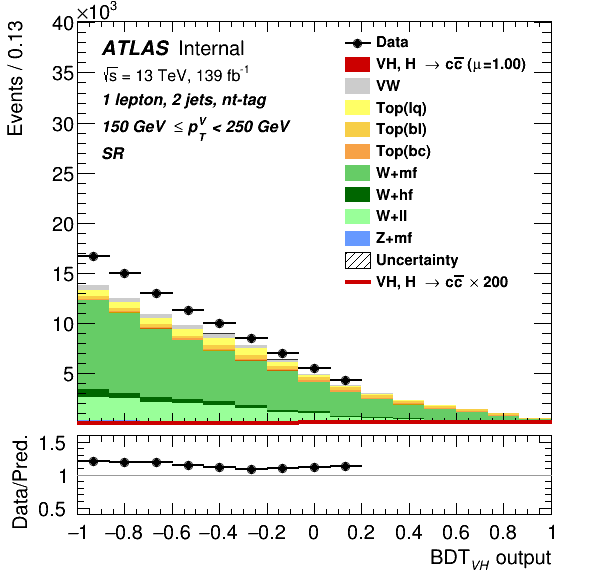
\includegraphics[width=0.32\textwidth]{Images/VH/SRsandTopCRs/Region_distmva_DSR_BMax250_L1_Y6051_TTypent_T1_J2_BMin150_Prefit.png}
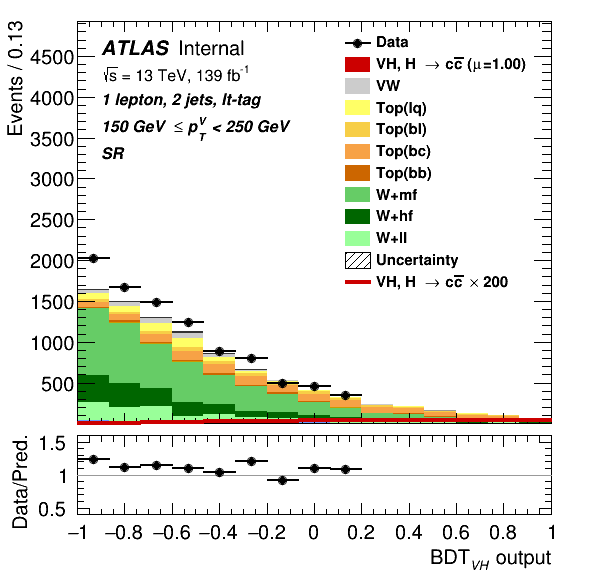
\includegraphics[width=0.32\textwidth]{Images/VH/SRsandTopCRs/Region_distmva_DSR_BMax250_L1_Y6051_TTypelt_T2_J2_BMin150_Prefit.png}
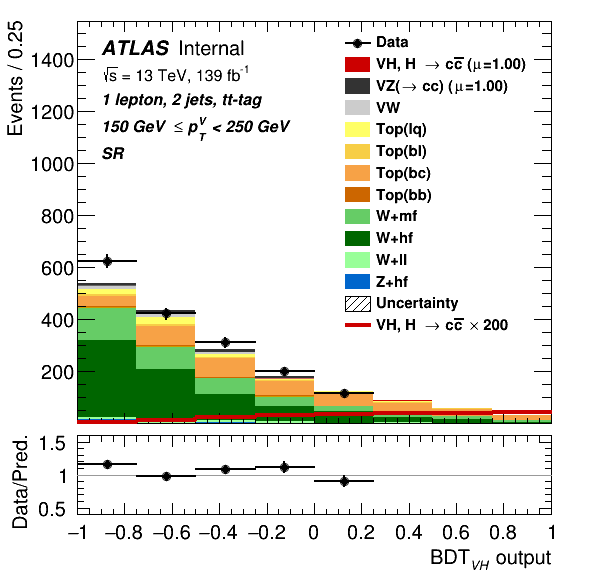
\includegraphics[width=0.32\textwidth]{Images/VH/SRsandTopCRs/Region_distmva_DSR_BMax250_L1_Y6051_TTypett_T2_J2_BMin150_Prefit.png}\\
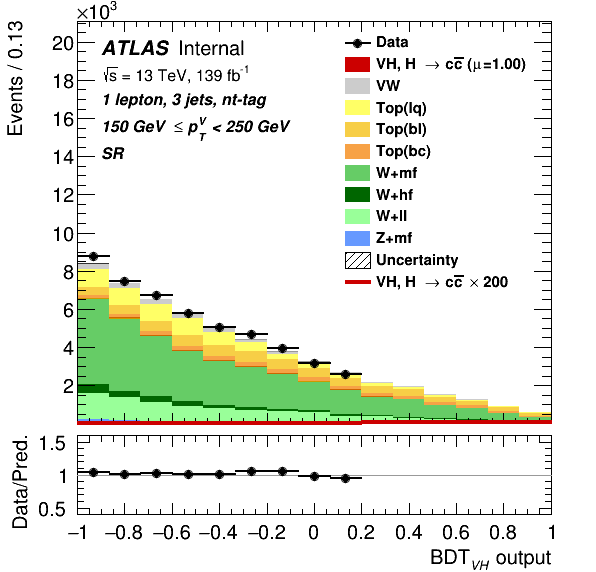
\includegraphics[width=0.32\textwidth]{Images/VH/SRsandTopCRs/Region_distmva_DSR_BMax250_L1_Y6051_TTypent_T1_J3_BMin150_Prefit.png}
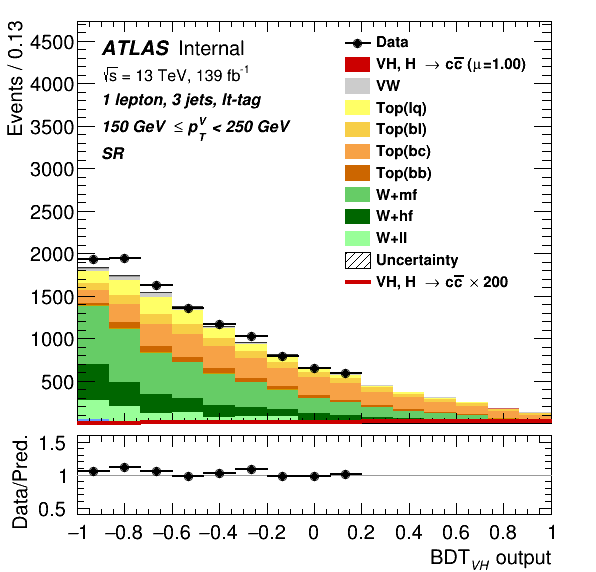
\includegraphics[width=0.32\textwidth]{Images/VH/SRsandTopCRs/Region_distmva_DSR_BMax250_L1_Y6051_TTypelt_T2_J3_BMin150_Prefit.png}
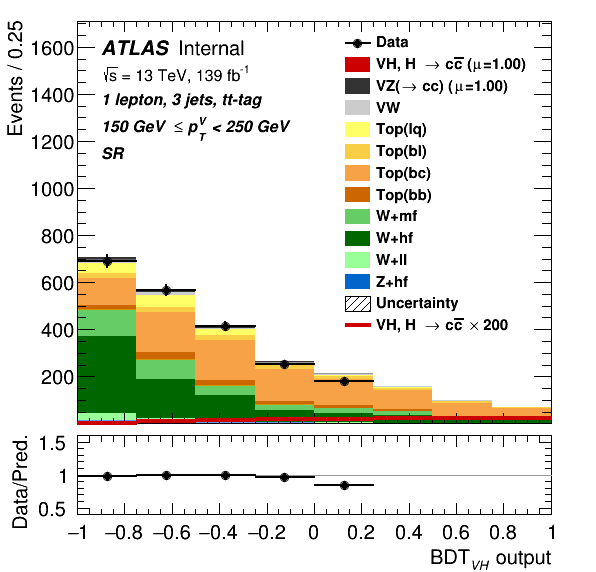
\includegraphics[width=0.32\textwidth]{Images/VH/SRsandTopCRs/Region_distmva_DSR_BMax250_L1_Y6051_TTypett_T2_J3_BMin150_Prefit.png}
\caption{The 1L signal regions BDT distributions in the low [150-250] $p_T^V$ range. Left: NT; centre: LT; right: TT. Top: 2 jets; bottom: 3 jets.} 
\label{fig:SRslowptv}
\end{figure}

The components contributing the most in the $VH(H\rightarrow c\bar{c})$ side of the analysis are the top($bc$) and top($bl$), due to the tagging requirement. There is very little top($bb$) thanks to the good performance of the tagger. Top($lq$) is mostly found in the looser tag regions (NT, LT) and not where the signal peaks. Figure \ref{fig:topCRslowptv} displays the new top control regions proposed in this work: as expected, the bulk of the distributions is made of top background, centred around the expected Higgs mass. The philosophy behind the proposed new design leverages the pseudo-continuous tagging to select the highest $p_T$ $b$-tagged and $c$-tagged jets as Higgs candidates. Thus, BL and BT regions are defined depending on whether the highest $p_T$ $c$-tagged jet is loose- or tight-tagged. The regions are further split in the number of jets and the same definition is used in the 0L channel. The full tag compositions of each region are as follows:

\begin{itemize}
\item 2-jet: \quad BL: $BL$;  \quad BT: $BT$
\item 3-jet:  \quad BL: $BLN$, $BLL$;  \quad BT: $BTN$, $BTL$, $BTT$, and $BBT$
\end{itemize}
In the \textit{AllSignal} strategy, the Higgs candidates in the topCR are always the highest $p_T$ $b$- and $c$-tagged jets. This selection was observed to make the top control region distributions more closely match the distributions in the signal regions. \\

\begin{figure}[h!]
\center
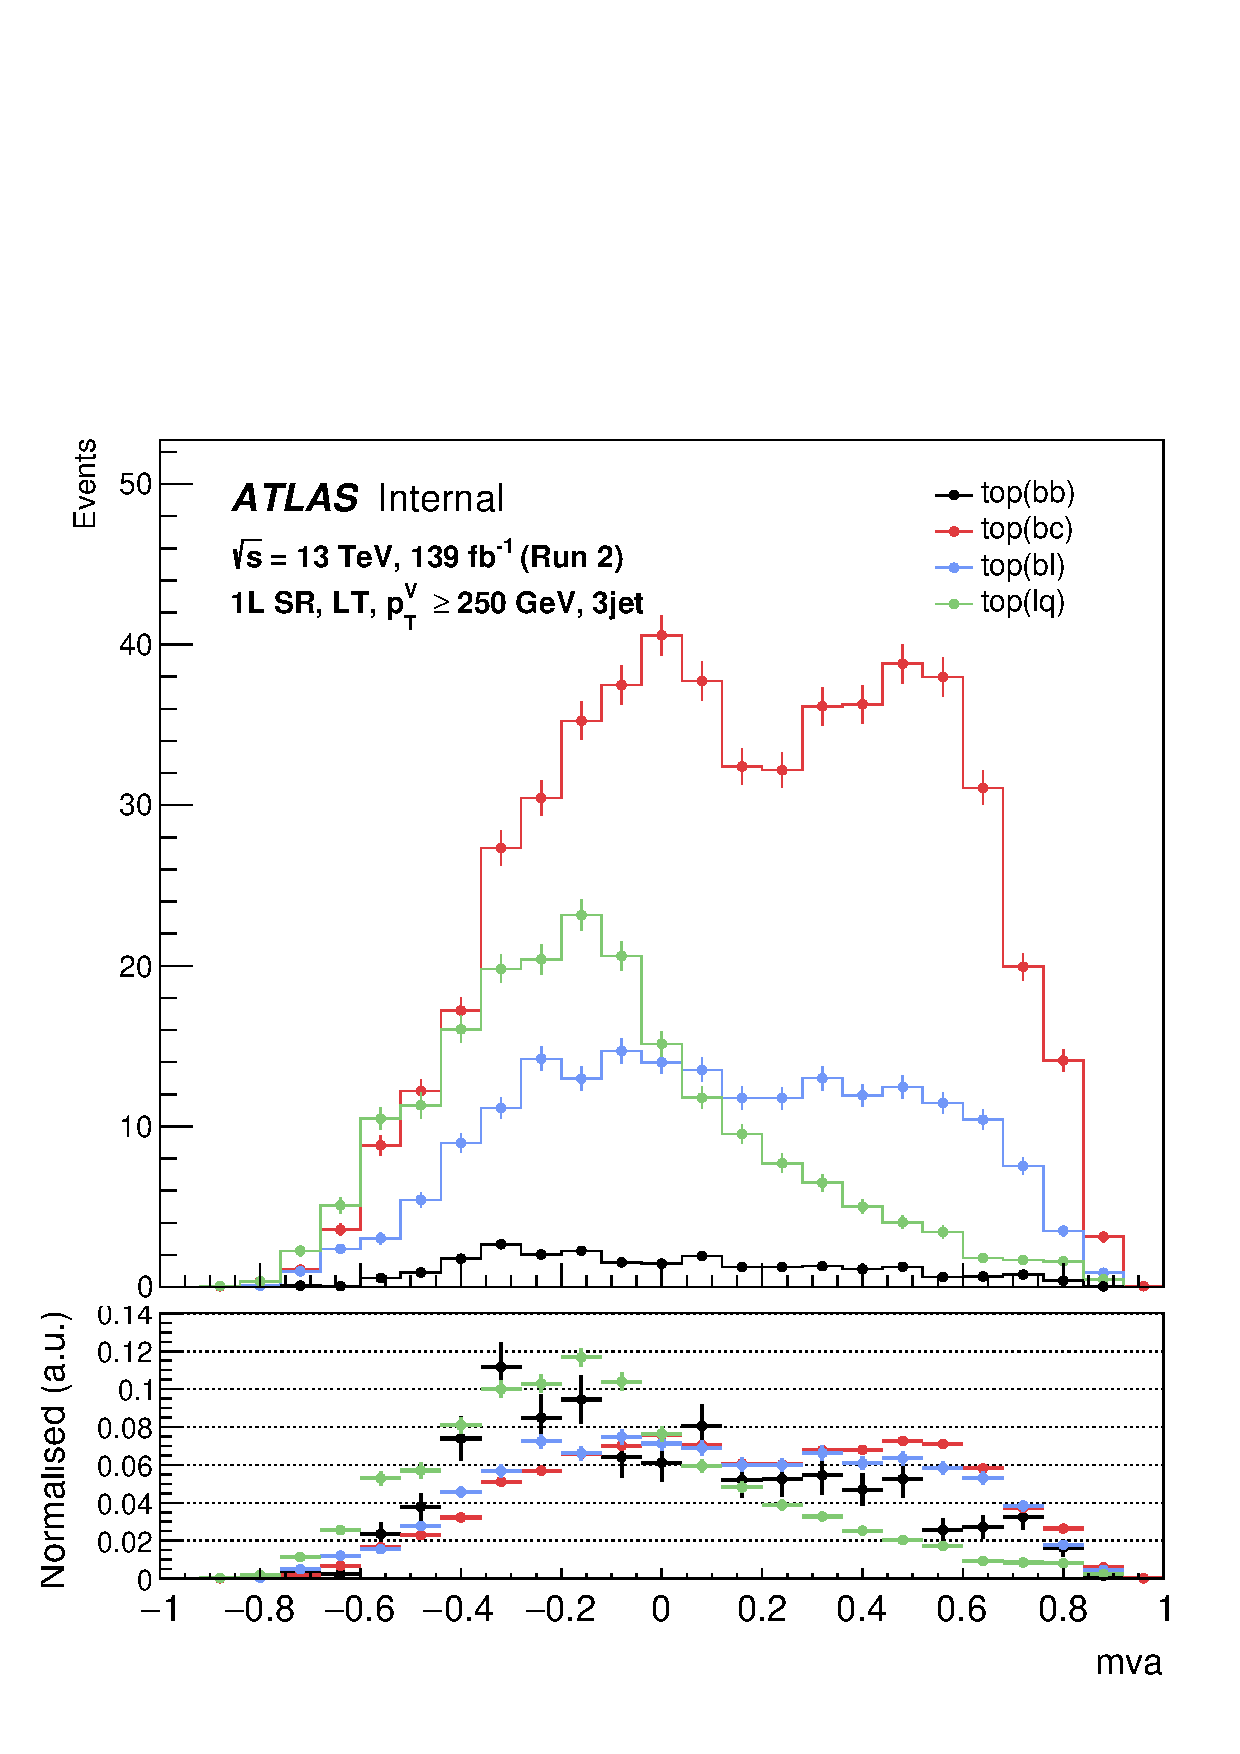
\includegraphics[width=0.48\textwidth]{Images/VH/top/OneLepton_top_2lttag3jet_SR_250ptv_mva.pdf}
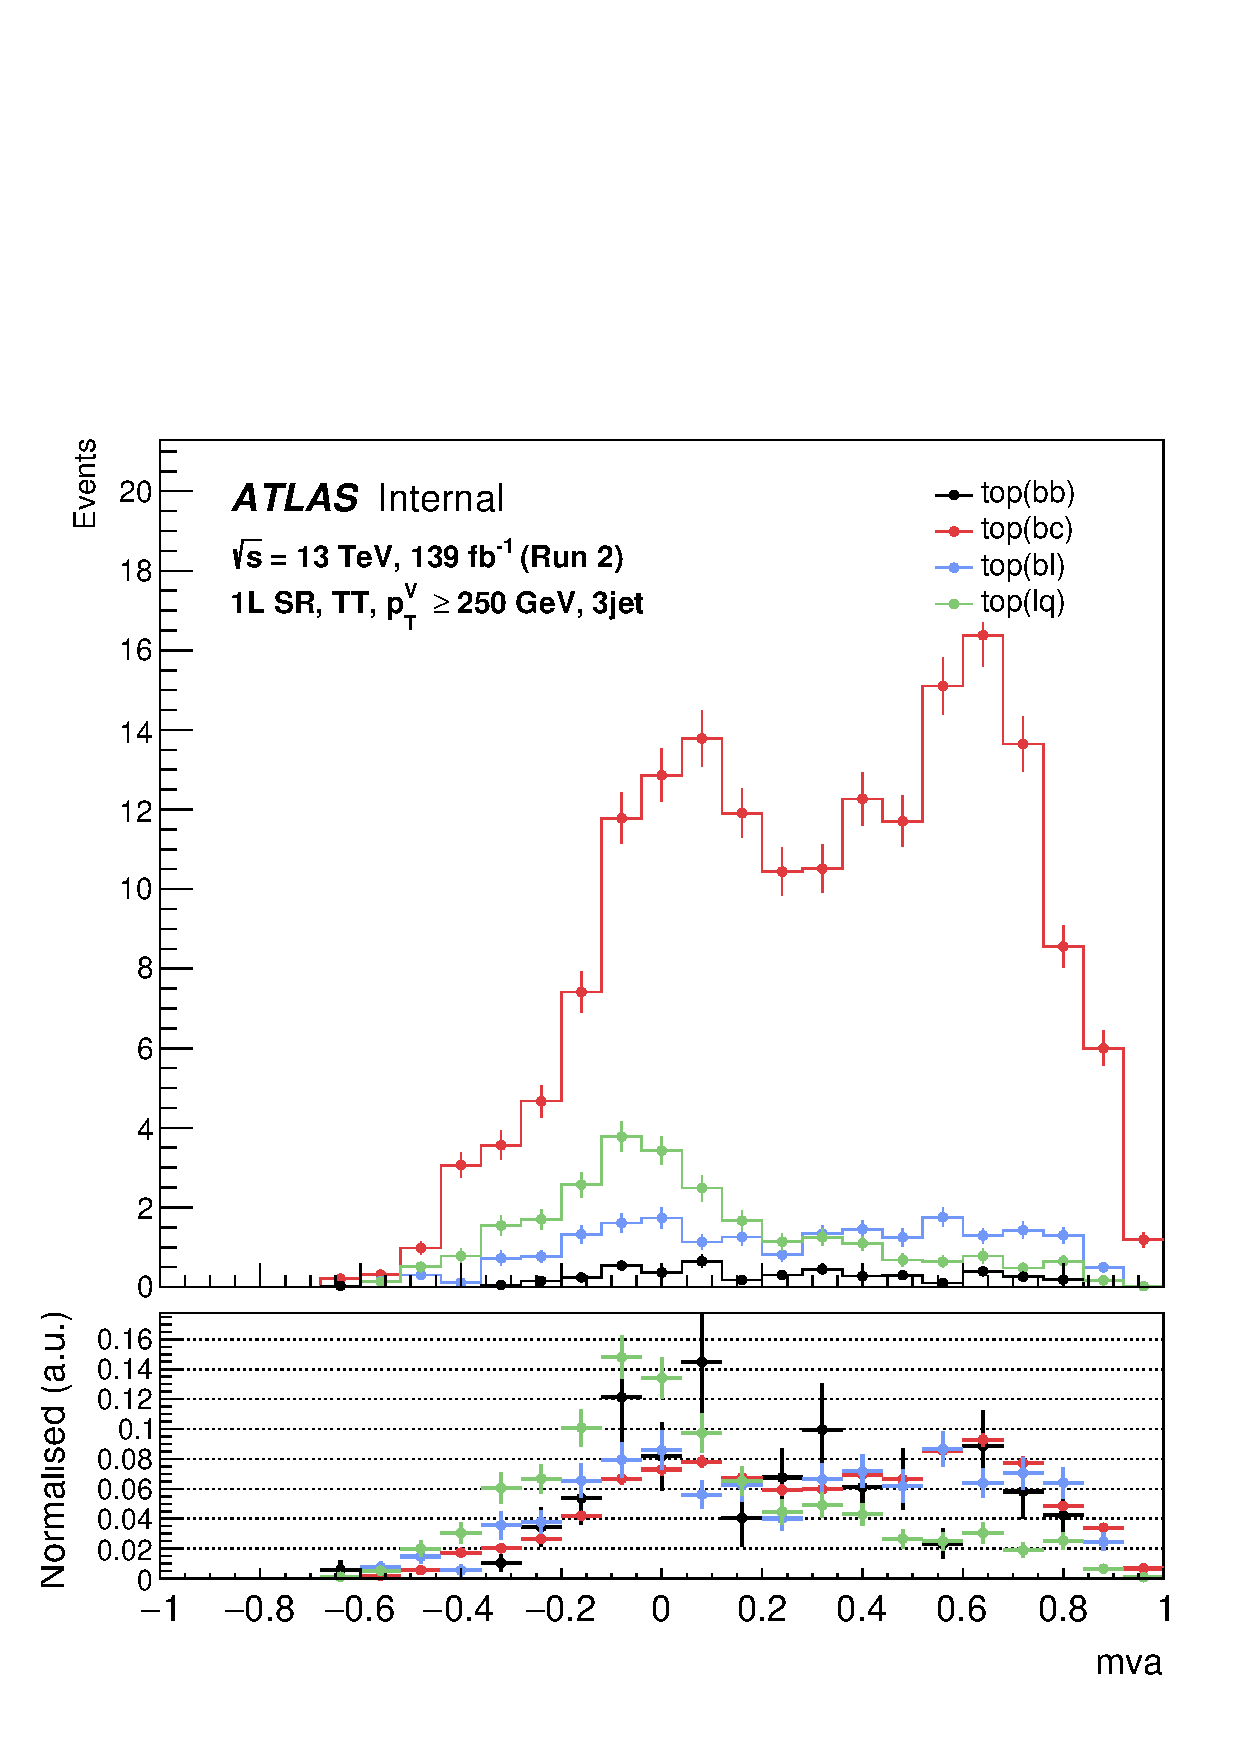
\includegraphics[width=0.48\textwidth]{Images/VH/top/OneLepton_top_2tttag3jet_SR_250ptv_mva.pdf}
\caption{Top components in the 1L 3 jets signal regions BDT distributions in the $\geq$ 250 GeV $p_T^V$ range. Left: LT; right: TT.}
\label{fig:topContentSR}
\end{figure}

\begin{figure}[h!]
%\hspace{-2.0cm}
\center
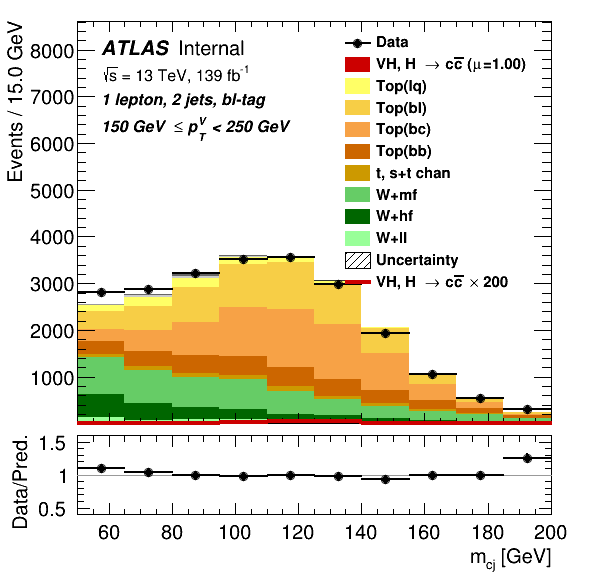
\includegraphics[width=0.24\textwidth]{Images/VH/SRsandTopCRs/Region_distmBB_DtopCRBL_BMax250_L1_Y6051_TTypebl_T1_J2_BMin150_Prefit.png}
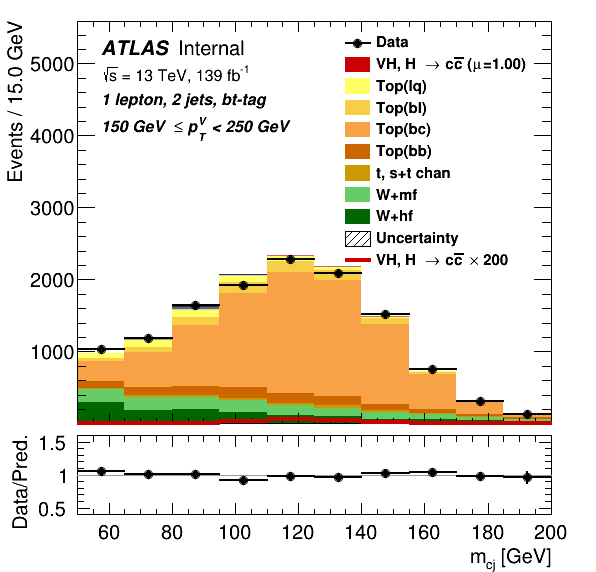
\includegraphics[width=0.24\textwidth]{Images/VH/SRsandTopCRs/Region_distmBB_DtopCRBC_BMax250_L1_Y6051_TTypebt_T1_J2_BMin150_Prefit.png}
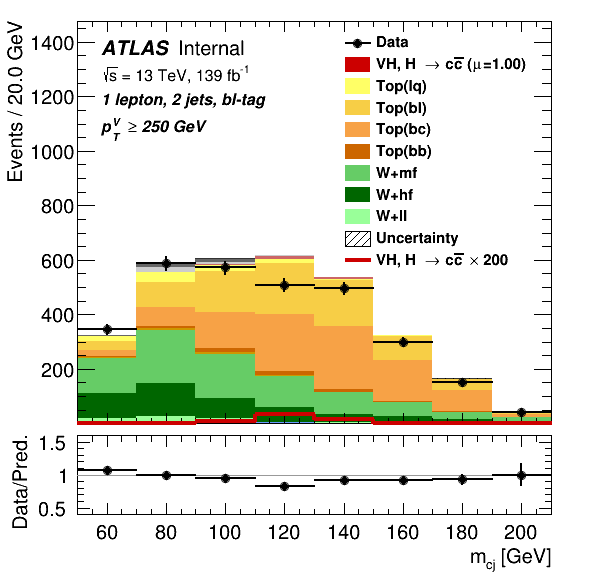
\includegraphics[width=0.24\textwidth]{Images/VH/SRsandTopCRs/Region_distmBB_DtopCRBL_L1_Y6051_TTypebl_T1_J2_BMin250_Prefit.png}
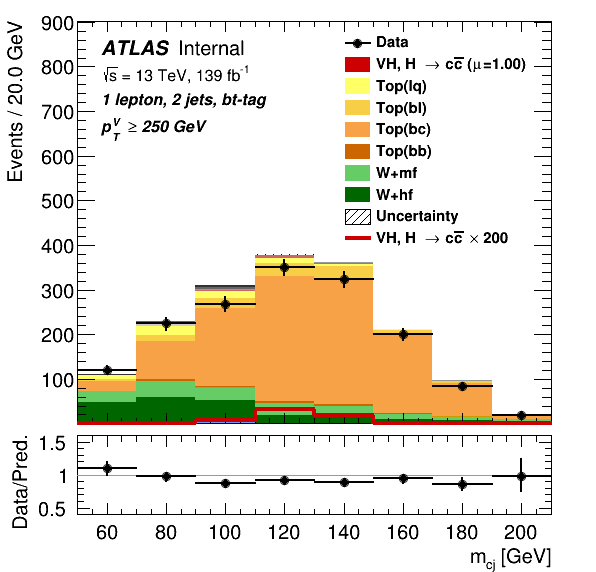
\includegraphics[width=0.24\textwidth]{Images/VH/SRsandTopCRs/Region_distmBB_DtopCRBC_L1_Y6051_TTypebt_T1_J2_BMin250_Prefit.png}\\

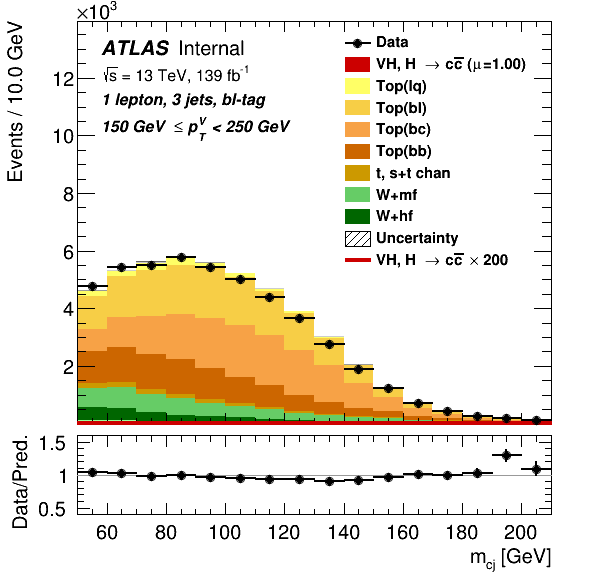
\includegraphics[width=0.24\textwidth]{Images/VH/SRsandTopCRs/Region_distmBB_DtopCRBL_BMax250_L1_Y6051_TTypebl_T1_J3_BMin150_Prefit.png}
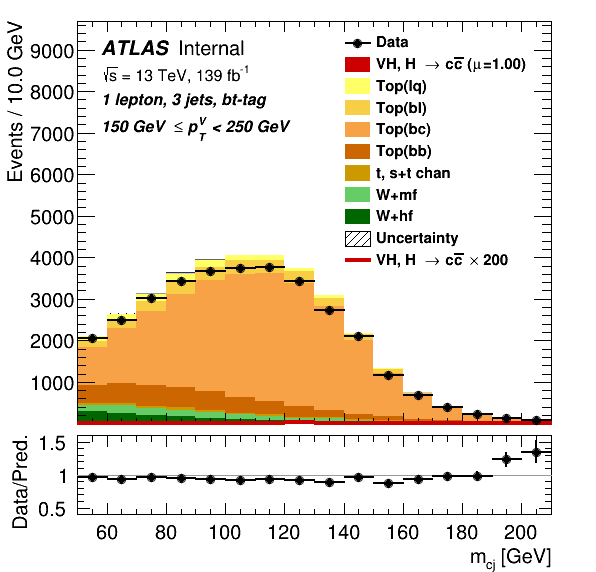
\includegraphics[width=0.24\textwidth]{Images/VH/SRsandTopCRs/Region_distmBB_DtopCRBC_BMax250_L1_Y6051_TTypebt_T1_J3_BMin150_Prefit.png}
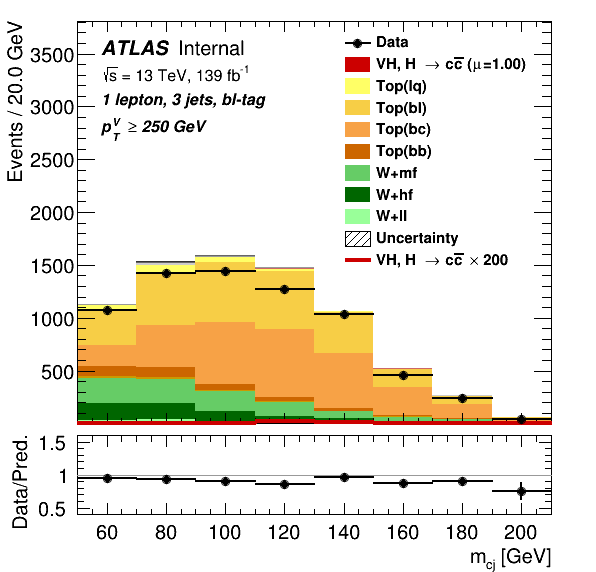
\includegraphics[width=0.24\textwidth]{Images/VH/SRsandTopCRs/Region_distmBB_DtopCRBL_L1_Y6051_TTypebl_T1_J3_BMin250_Prefit.png}
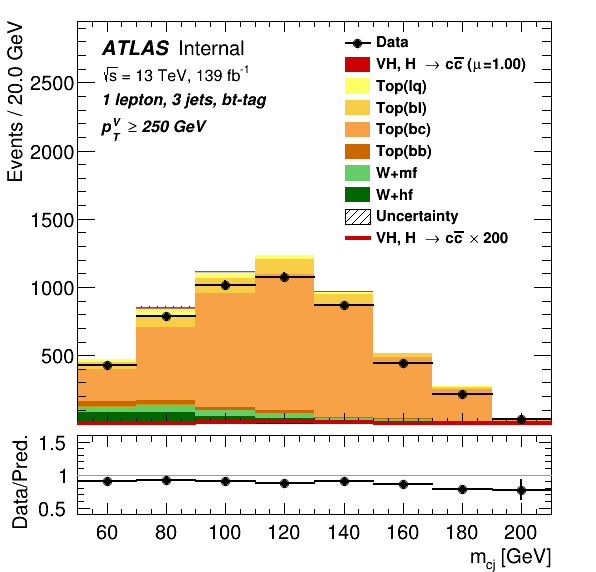
\includegraphics[width=0.24\textwidth]{Images/VH/SRsandTopCRs/Region_distmBB_DtopCRBC_L1_Y6051_TTypebt_T1_J3_BMin250_Prefit.png}
\caption{The 1L top control regions $m_{c\bar{c}}$ distributions in both $p_T^V$ ranges (left two columns are [150, 250] GeV, right two are > 250 GeV). Per group of two adjacent: left is BL, right is BT. Top: 2 jets; bottom: 3 jets.} 
\label{fig:topCRslowptv}
\end{figure}

\begin{figure}[h!]
\center
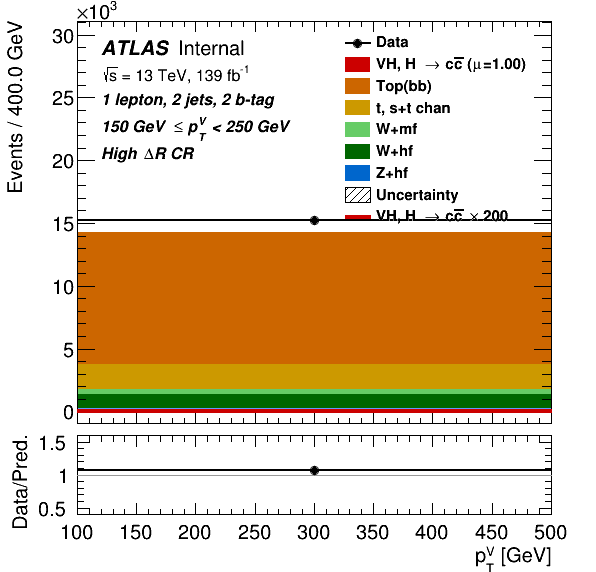
\includegraphics[width=0.48\textwidth]{Images/VH/SRsandTopCRs/Region_distpTV_DCRHigh_BMax250_L1_Y6051_TTypebb_T2_J2_BMin150_Prefit.png}
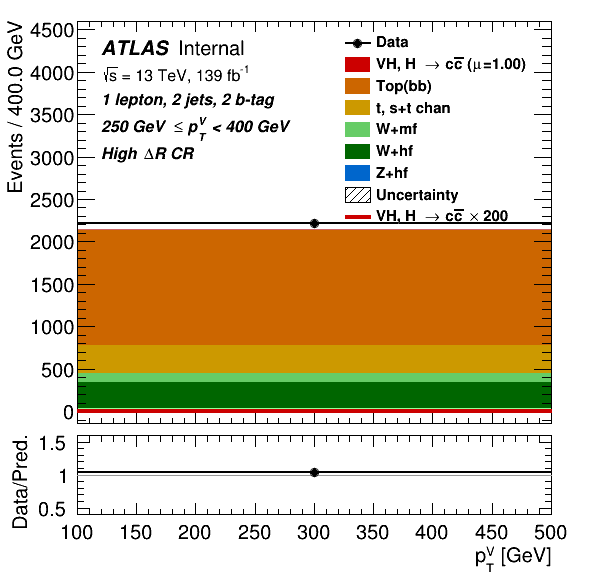
\includegraphics[width=0.48\textwidth]{Images/VH/SRsandTopCRs/Region_distpTV_DCRHigh_BMax400_L1_Y6051_TTypebb_T2_J2_BMin250_Prefit.png}\\
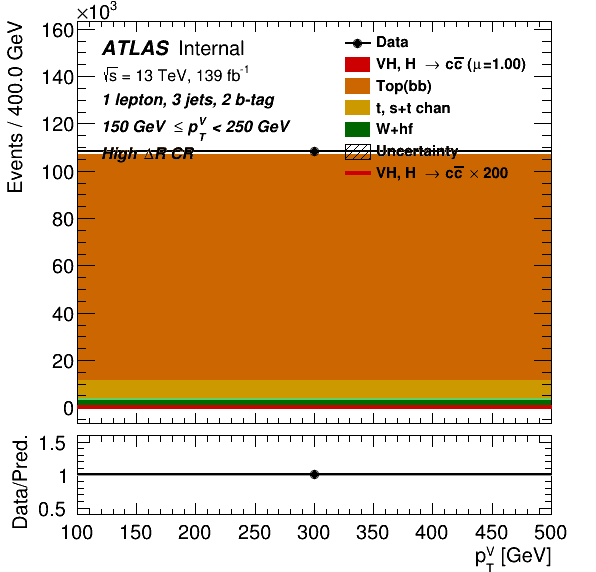
\includegraphics[width=0.48\textwidth]{Images/VH/SRsandTopCRs/Region_distpTV_DCRHigh_BMax250_L1_Y6051_TTypebb_T2_J3_BMin150_Prefit.png}
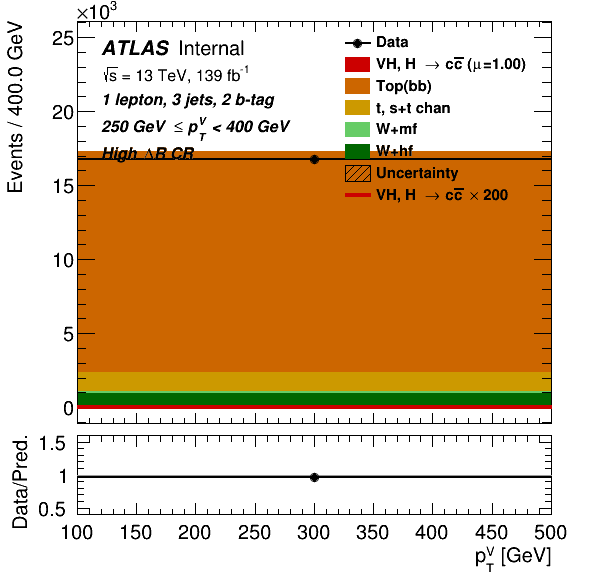
\includegraphics[width=0.48\textwidth]{Images/VH/SRsandTopCRs/Region_distpTV_DCRHigh_BMax400_L1_Y6051_TTypebb_T2_J3_BMin250_Prefit.png}
\caption{The 1L 1-bin  $VH(H\rightarrow b\bar{b})$ High $\Delta R$ CR in both $p_T^V$ ranges. Left: [150, 250] GeV; right: [250, 400] GeV. Top: 2 jets; bottom: 3 jets.} 
\label{fig:vhbbDRCR}
\end{figure}

\begin{figure}[h!]
%\hspace{-2.0cm}
\center
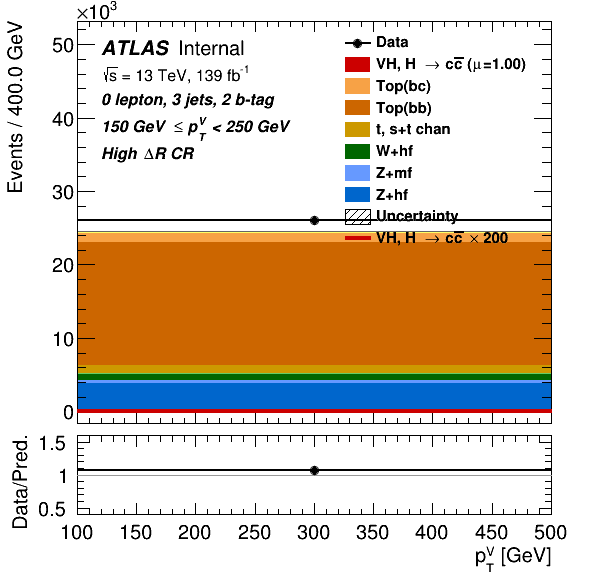
\includegraphics[width=0.48\textwidth25]{Images/VH/SRsandTopCRs/Region_distpTV_DCRHigh_BMax250_L0_Y6051_TTypebb_T2_J3_BMin150_Prefit.png}
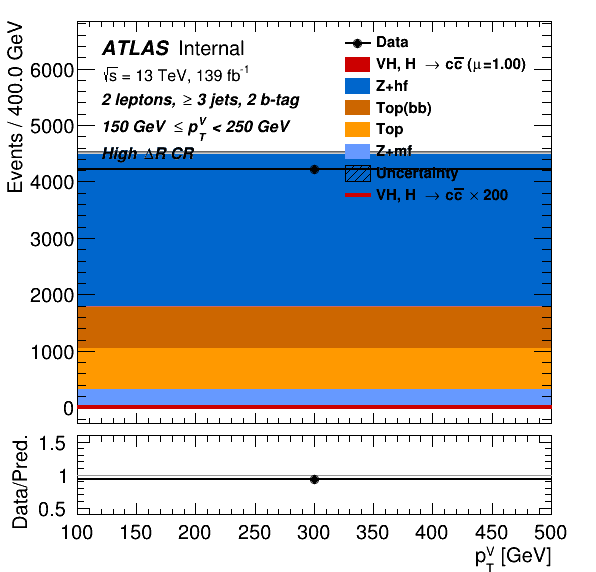
\includegraphics[width=0.48\textwidth25]{Images/VH/SRsandTopCRs/Region_distpTV_DCRHigh_BMax250_BMin150_Y6051_TTypebb_T2_J3_L2_incJet1_Prefit.png}
\caption{The $VH(H\rightarrow b\bar{b})$ High $\Delta R$ CR in the [150, 250] GeV $p_T^V$ range region with 3 jets, for 0L on the left, and 2L on the right.} 
\label{fig:vhbbDRCR02L}
\end{figure}

For $VH(H\rightarrow c\bar{c})$, the $bc$ and $bl$ components are the most important to constrain. In $VH(H\rightarrow b\bar{b})$, while the $bc$ component is also significant and can benefit from the topCRs, the most important contribution comes from the $bb$ one and is well constrained by the High $\Delta R$ CR, since in a $t\bar{t}$ decay the two produced $b$-jets tend to be separated by a large $\Delta R$ due to the event topology. For the Combined Analysis, the SRs and CRs of both analyses will be considered simultaneously. To show the impact on the $VH(H\rightarrow c\bar{c})$ standalone analysis, the High $\Delta R$ CR from  $VH(H\rightarrow b\bar{b})$ is included to study the effect on the $bc$ and $bl$ components. The aim is to demonstrate these and the $bb$ component can be well constrained with these regions alone, and in particular without the SRs of $VH(H\rightarrow b\bar{b})$. The $VH(H\rightarrow b\bar{b})$ High $\Delta R$ control regions are taken as a single bin of $p_T^V$, because the interest is solely to constrain the top($bb$) normalisation. Figure \ref{fig:vhbbDRCR} displays the 1L $VH(H\rightarrow b\bar{b})$ High $\Delta R$ CR, which is visibly dominated by the top($bb$). Figure \ref{fig:vhbbDRCR02L} shows the same region for the [150, 250] GeV $p_T^V$ range with 3 jets in 0L and 2L, showing a significant proportion of $Z$+jets is also included in these regions.  \\
